\chapter{Methodology and Results}

The previous section outlined the procedure for using Bayesian inference to solve a simple regression problem. It then expanded the concept to allowing for regression where the data is not in the same space as the inference result. The two spaces being connected by a forward model or responce matrix. This is exactly what is required as interferometry data is not in the same space as the profile to be inferred. Two main methods for dealing with the hyperparameters were also outlined. They are \gls{map} and marginalisation. Results will be presented for both sections. Both allow for hyperpriors to be included. A uniform prior is used for all hyperparameters and the bounds were selected by carefully observing how the parameters affect the resulting inferrence and allowing generous amount of room for profile extreamities to exist. The amplitude is contrained to between $0$ and $100$ and is on the same scale as the electron density $\cdot 10^{20}$. Each length scale is bounded between 0 and 3 and is on the same scale as the normalised radius. This includes the non static kernel varients hyperbolic tangent length scale and cubic spline length scale. 5 knots were used for the cubic spline. To reduce the dimensionality of the problem they were evenly spaced across the normalised radius. Each interferometry channel is assumed to have the same experimental error and it is bounded between $0.03$ and $0.05 \, \cdot10^{-19}m^2$. WEST reports a no plasma noise in the order of $0.03 \cdot10^{-19}m^2$. The hyperparameter \gls{map} is found by minimising the loss function based on the marginal likelihood, see equation \ref{eq:loss}. When any trialed parameters exceed their prior bounds the loss returns infinity (or a very high number). SciPy minimise and PyTorch SGD are both gradient based methods that were trialed and achieved similar results. In order to precisely measure the accuracy of the inferences a known ground truth profile is required. The metric used is mean square error and is included on each graph as `mse'. There are a few main profile types of interest to the scientific community. L mode or low confinement profiles are typically parabolic like in shape and are the bread an butter of takamak operation. It is the easiest profile to achieve and is often a stepping stone to achiving other profiles within a plasma shot. This is the main profile used within the \gls{west} tokamak. H mode or high confinement mode is achieved by increasing external heating power from sources such as neutral bean injection and electron cyclotron resonance heating. H mode profiles have a distinct sharp drop in density near the plasma boundary. H mode profiles are well known for largely increasing the energy confinement time of the plasma which is a cruicial factor for net positive energy production. Although they do introduce extra instabilites known as ELMS. Another interesting profile feature is known as peaking. The external heating elements can be tuned to target the core. The extra heat ionises more of the fuel and decreases electrion-ion recombination rates. This increases the electron density in the core and creates a peak or bell shape profile. This can be achieved with both L mode and H mode. Peaking is known to increase the stability and performance of the plasma. It helps reduce the impurities in the core that contribute to radiation loss. Versions of these profiles are shown in figure \ref{fig:groundtruth}. The interferomety data that would be measured given a profile as the ground truth is computed with the responce matrix. The responce matrix is created using real magnetic field lines inffered by NICE. A generously small Gaussian experimental error is added with a standard deviation of $3\cdot10^-17 \, m^2$. This is what \gls{west} reports the no plasma noise of the interferometer to be.  

\begin{figure}[ht]
    \centering
    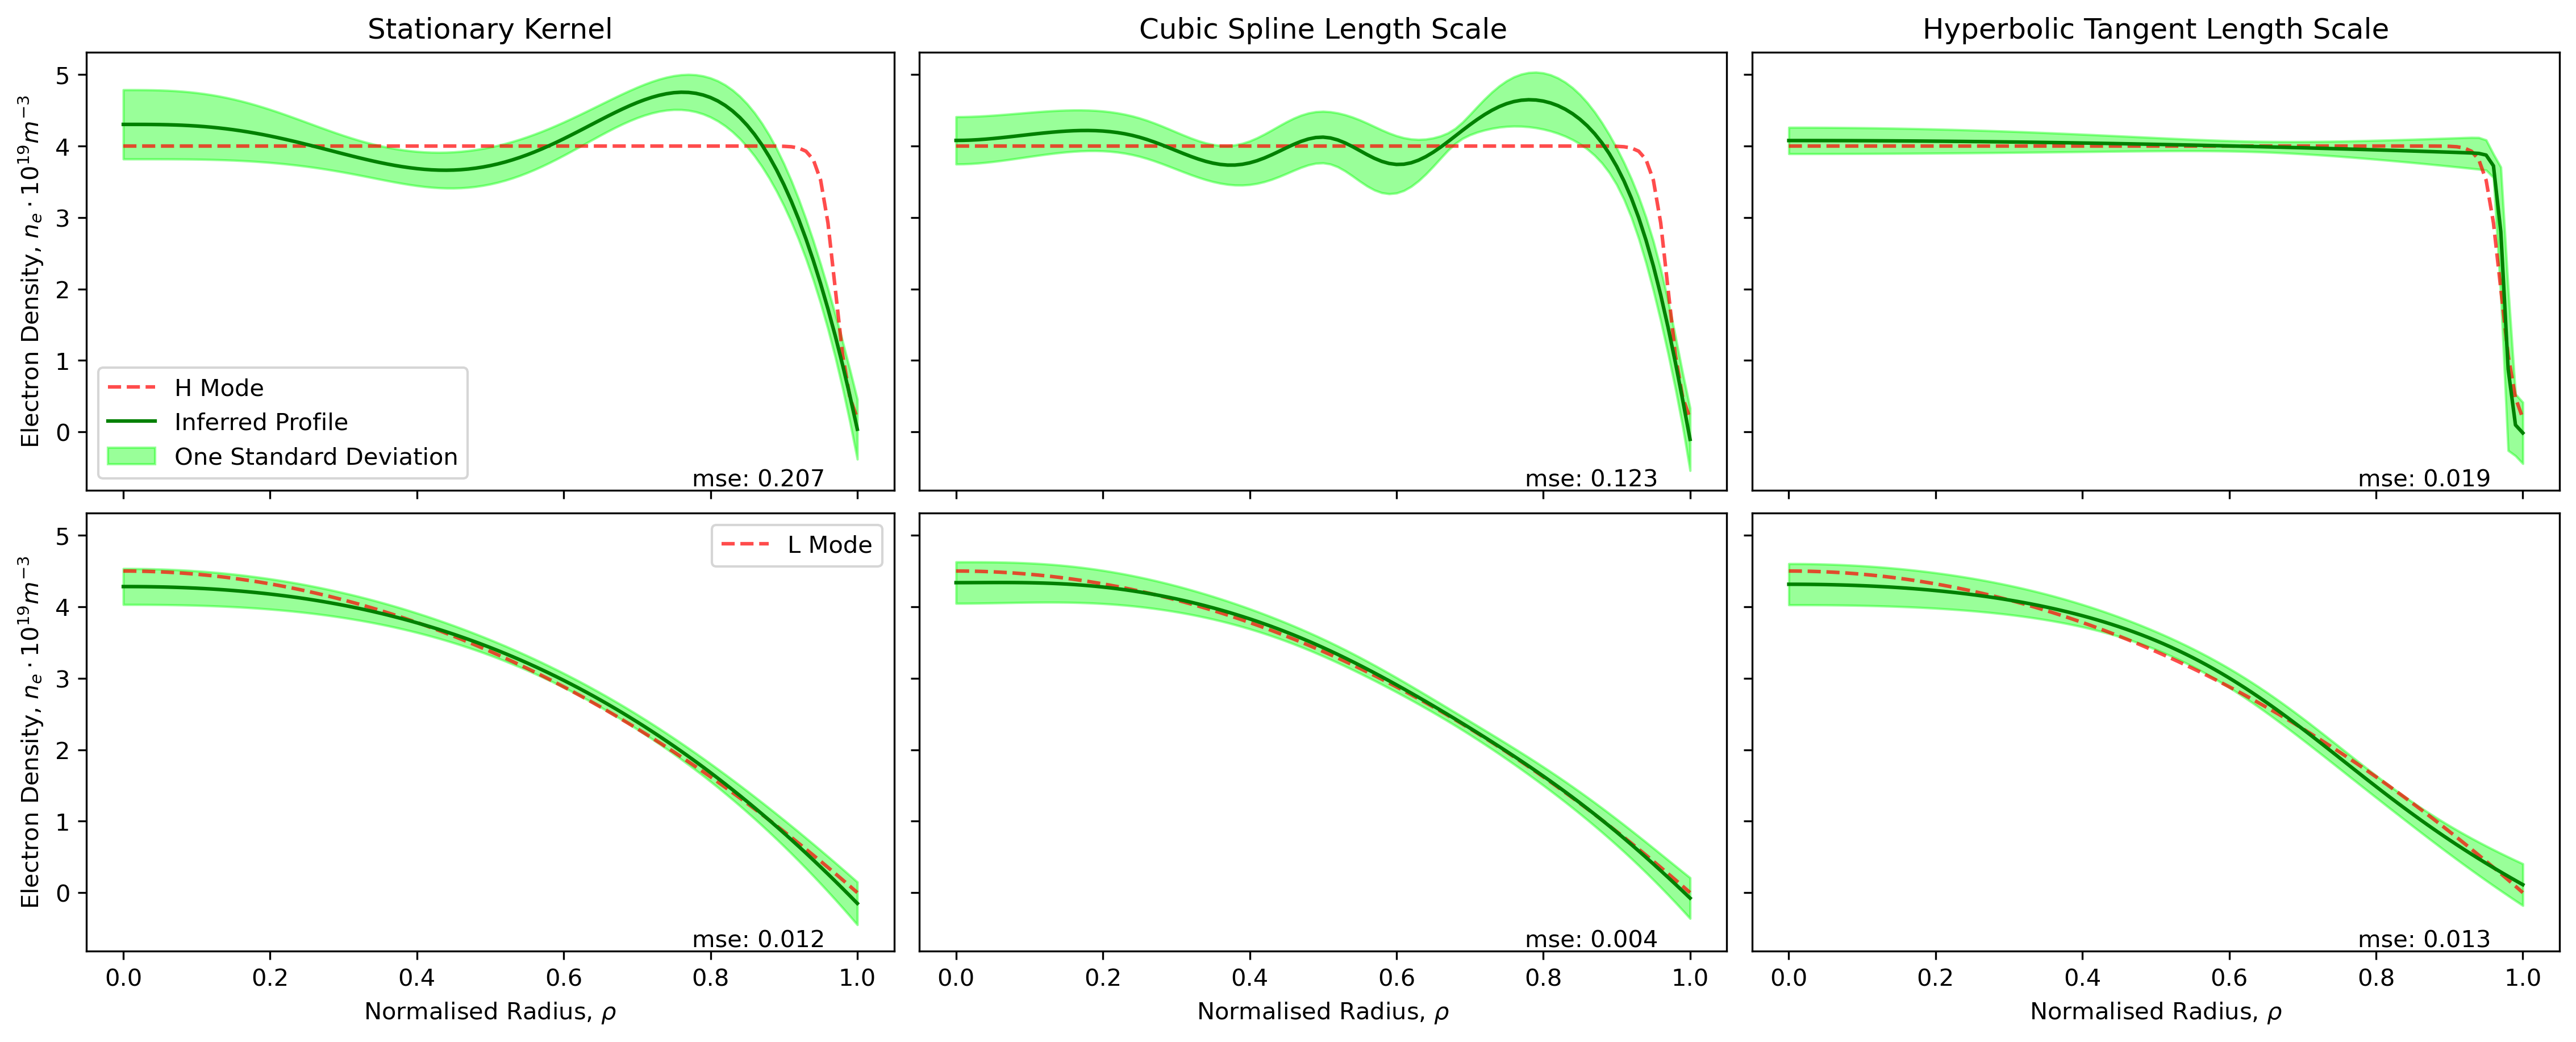
\includegraphics[width=10cm, angle=90]{images/Final/MAPsynthetic_final_hl.png}
    \caption{Ground truth profiles used to generate synthetic interferometry data.}
    \label{fig:groundtruth}
\end{figure}

\begin{figure}[ht]
    \centering
    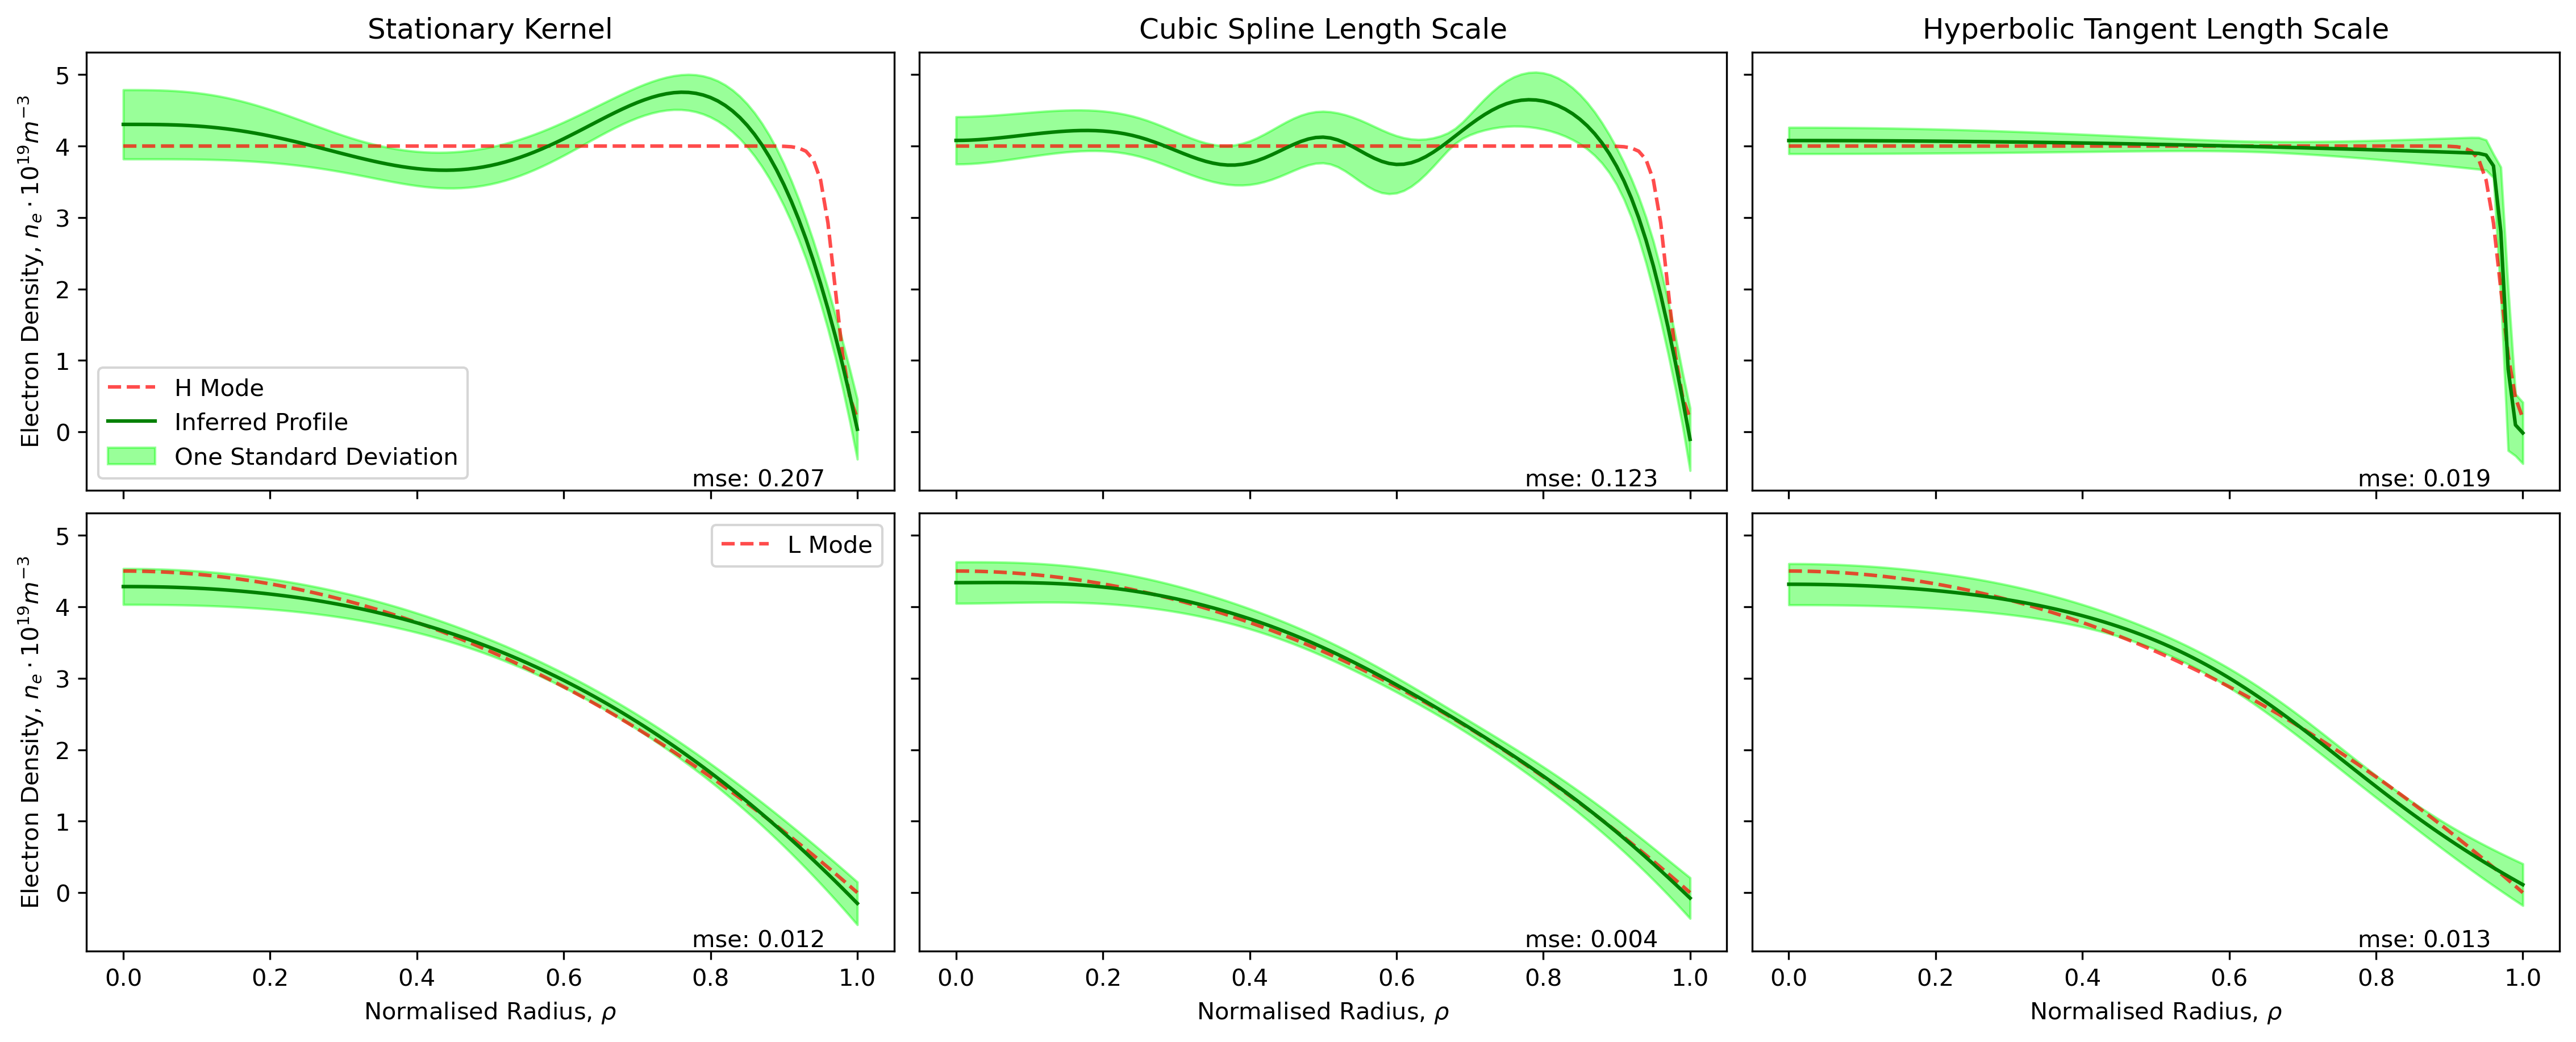
\includegraphics[width=10cm, angle=90]{images/Final/MAPsynthetic_final_hl.png}
    \caption{Electron density inference using the hyperparameter MAP method on synthetic interferometry data.}
    \label{fig:mapsynthetic}
\end{figure}

\begin{figure}[ht]
    \centering
    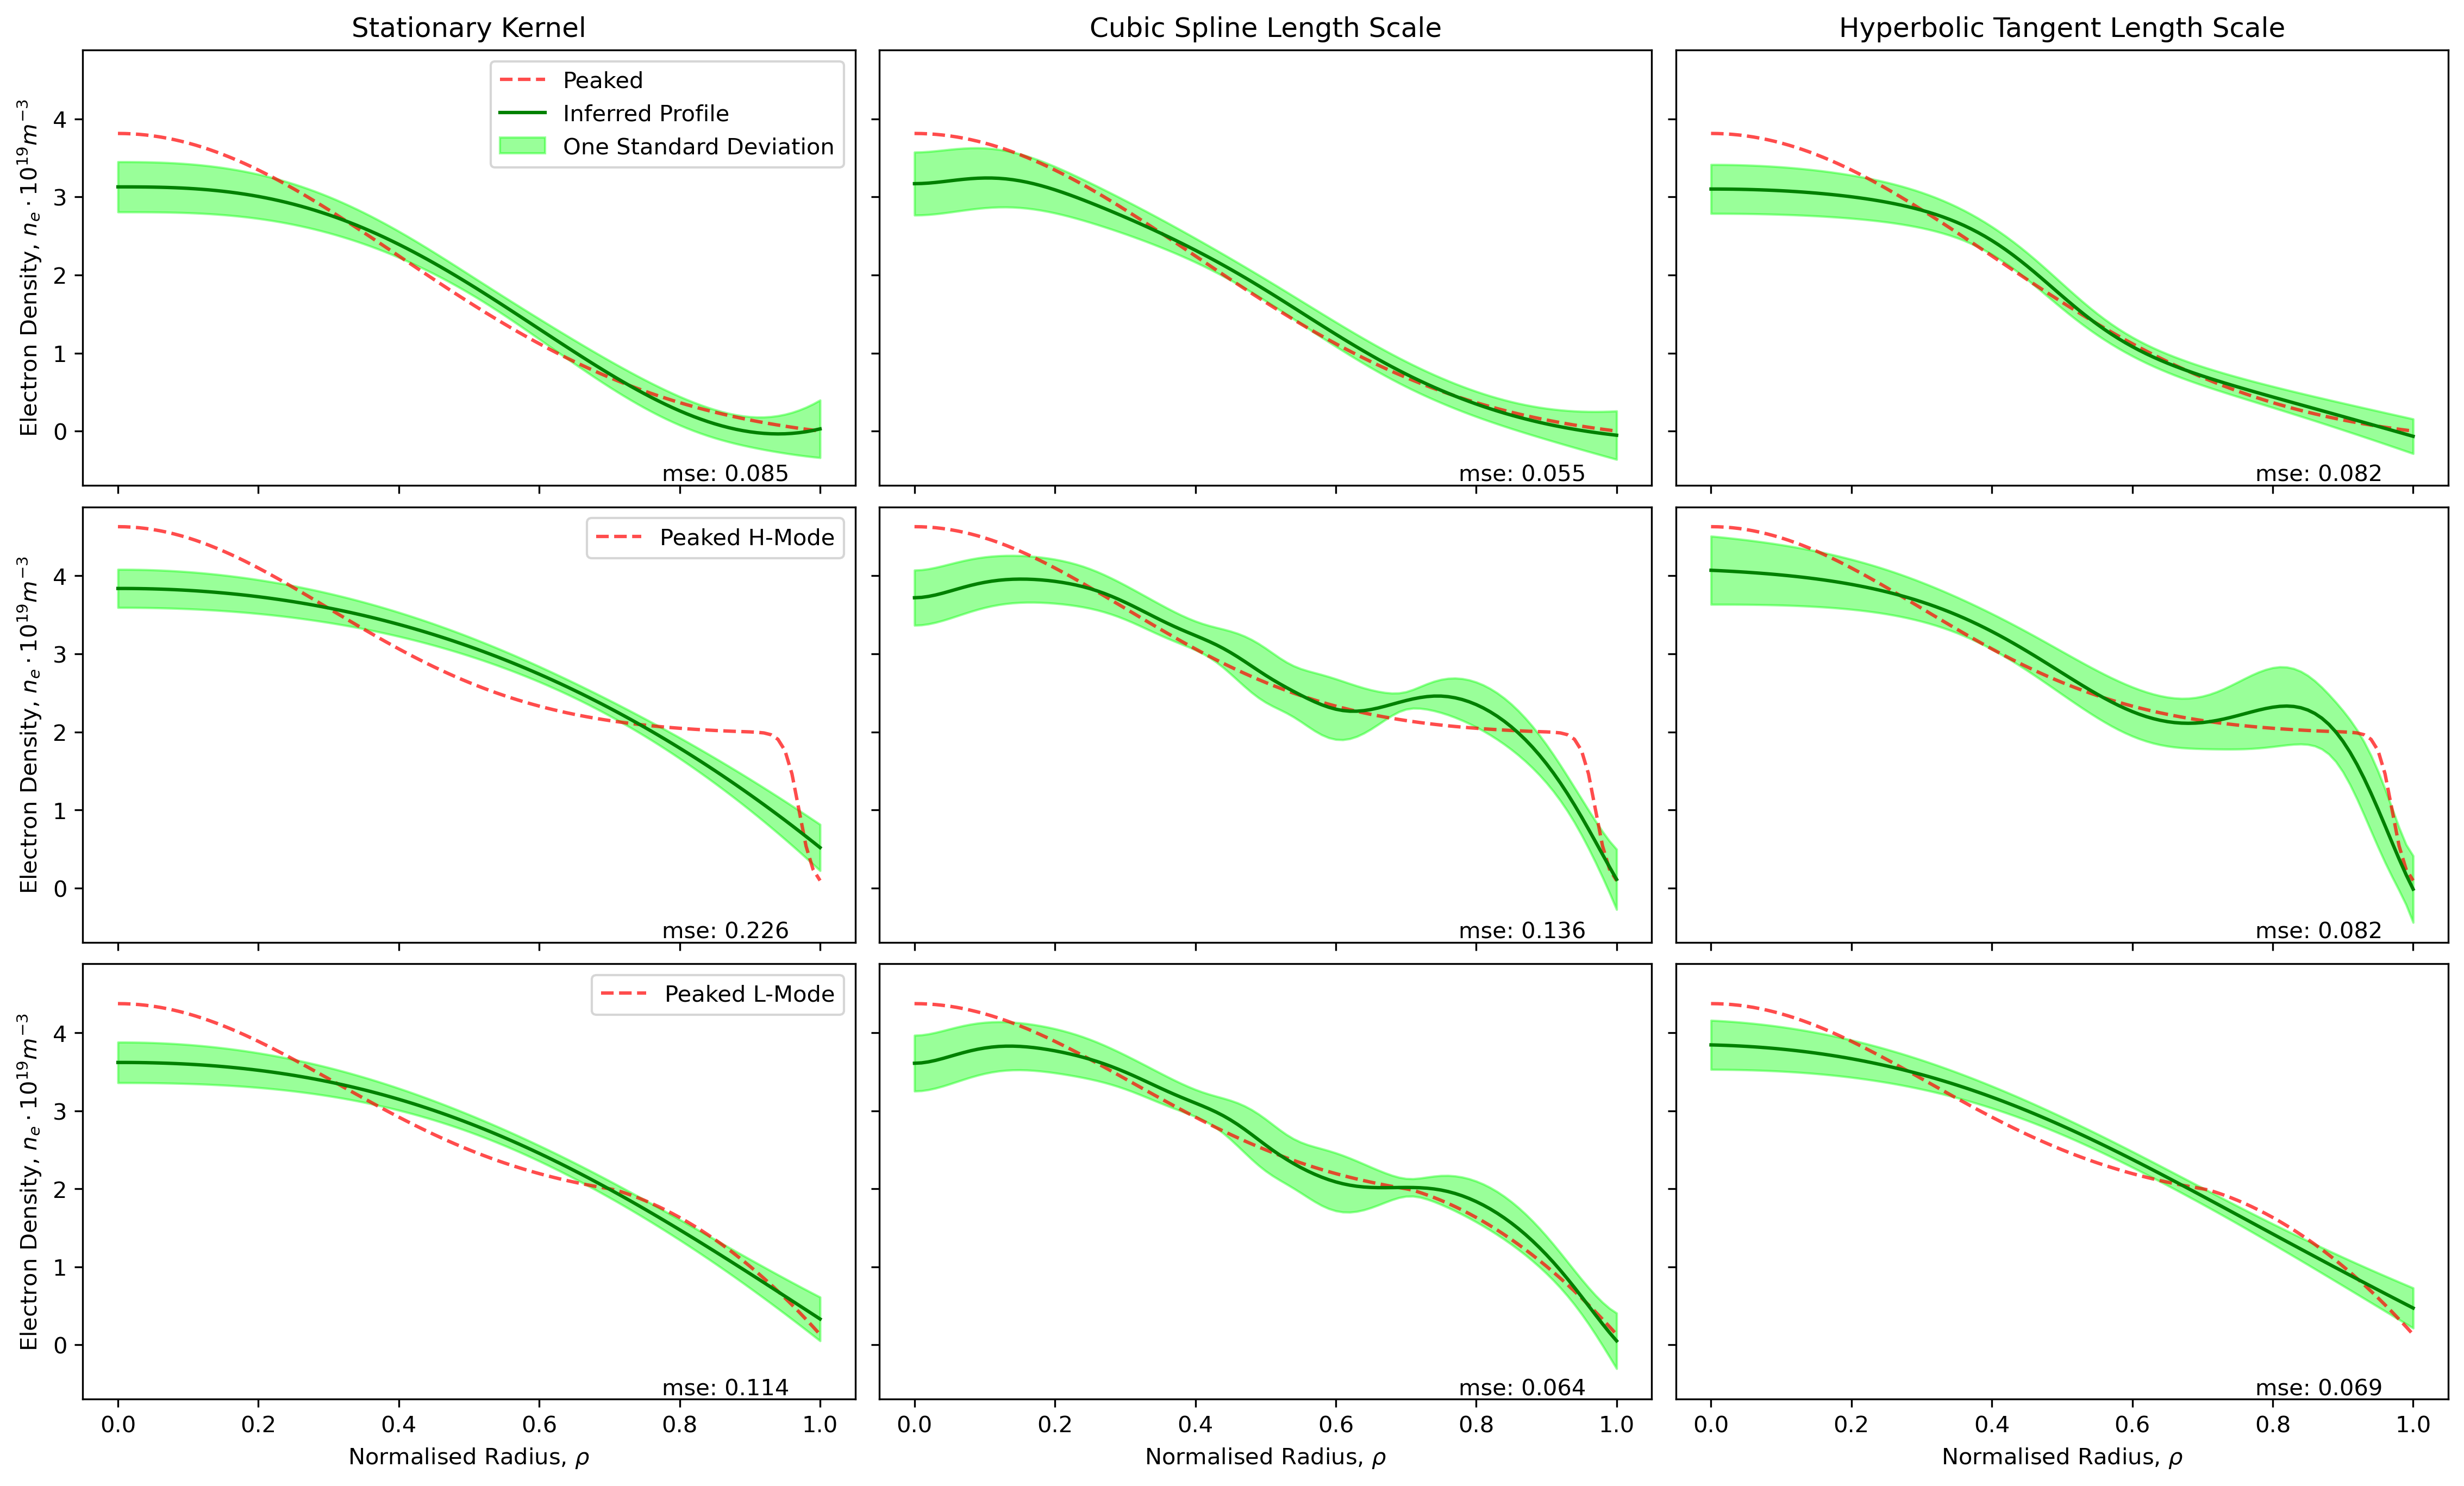
\includegraphics[width=10cm, angle=90]{images/Final/MAPsynthetic_final_p.png}
    \caption{Electron density inference using the hyperparameter MAP method on synthetic interferometry data.}
    \label{fig:mapsynthetic}
\end{figure}

% \begin{table}
% \centering
% \begin{tabular}{|c|c|c|}
%     \hline
%     \textbf{Hyperparameter} & \textbf{Lower Bound} & \textbf{Upper Bound} \\
%     \hline
%     Amplitude & 0 & 100 \\
%     Length Scale & 0 & 3 \\
%     \hline
%     \textbf{Hyperbolic Tangent} & &\\
%     Transition Center & 0 & 1 \\
%     Transition Width & 0.01 & 0.5 \\
%     \hline
%     \textbf{Cubic Spline} & & \\
%     5 Knots Evenly Spaced in $rho$ & & \\
%     \hline
% \end{tabular}
% \caption{}
% \label{tbl:prior}
% \end{table}

%methodology

% Explain the details of the how the theory is implimented, what processing power is required, I used python jupyter notebooks numpy, scipy and pytorch. Explain the key parts of the code in order to compute the kernels, marginal likelyhood and inference. What test were done in order to try and improve the inference. 

% \begin{itemize}
%     \item What format was the data in when it came from west and how did I import it into python
%     \item A bit about the diffent forms the data comes in on the west imas database and which one was chosen. 
%     \item How can the accuracy of the forward model be tested and how should this effect the experimental error.
%     \item How does one select an experimental error, is it important for the inference? 
%     \item What is the non positive definite matrix error, how can it be avoided, what are the implications of this
%     \item How I used meshgrid to compute the kernel in a fast way
%     \item what are the different methods used for finding the minimum of the marginal likelyhood, scipy minimize, pytorch, grid search. How do they work. 
%     \item What distributions did I use to randomly initialize the kernel parameters. Why did I randomly initialise them?
%     \item Why I coded everything with pytorch tensors
%     \item How I optimised the learning rate
%     \item Attempts to use noise
%     \item How did I try and improve the inference.
%     \item summarise the chapter and lead into the results. 
    
% \end{itemize}


% \begin{itemize}
%     \item Make the case as why a 0 mean prior is not always a good Idea, since the marginal likelyhood is not perfect and inferences favour the lower side of NICE, likely due to the 0 prior as when amp is increased the inference will move to NICE but not beyond it. Including prior knowledge when available is always advised.
    
%     \item Make the case that if I set NICE as the true ground truth and create synthetic data then I get the NICE profile from lowering marginal likelyhood. This shows that everything is set up correctly.
    
%     \item Show I am getting a local minimum of the marginal likelihood which is nice like and a lower minimum which is parabolic. This could be a result of the marginal likelihood not being a perfect loss function for problems with little data. This seems to be true for SciPy, PyTorch, static and non-static.
%     \item Talk about the discovered more defined ridge, ask for access to log book to see if this is during a H-mode shot. Explain why it might be physically significant but a full monte carlo bayesian should be carried out to verify this. 
%     \item Show the static grid search

%     \item Results not yet curated
%         \subitem Bayesian inference using monte carlo methods
%         \subitem One size fits all kernel for real time. 
%     \item summarise the chapter and lead into conclusions
% \end{itemize}